%
% loesung.tex -- Lösung von Bernoulli
%
% (c) 2021 Prof Dr Andreas Müller, OST Ostschweizer Fachhochschule
%
\bgroup
\pgfmathparse{12/(2*3.1415)}
\xdef\r{\pgfmathresult}
\def\zentrum#1{ ({12*#1/360},{-\r}) }
\def\zykloide#1{ 
	({(12*#1/360)-\r*sin(#1)},{\r*(cos(#1)-1)})
}
\def\kreis#1{
	\fill[color=blue!50,opacity=0.5] \zentrum{#1} circle[radius=\r];
	\fill[color=blue!50,opacity=0.7] \zentrum{#1}
		-- ++(0,{0.5*\r}) arc (90:{90+#1}:{0.5*\r}) -- cycle;
	\draw[color=blue!50,opacity=0.7] \zentrum{#1} -- ++(90:\r);
	\draw[color=blue,line width=1.6pt] \zentrum{#1} -- \zykloide{#1};
	\fill[color=blue!50] \zentrum{#1} circle[radius=0.08];
	\fill[color=blue] \zykloide{#1} circle[radius=0.1];
}
\begin{frame}[t]
\setlength{\abovedisplayskip}{5pt}
\setlength{\belowdisplayskip}{5pt}
\frametitle{Zykloide}
\vspace{-10pt}
\begin{center}
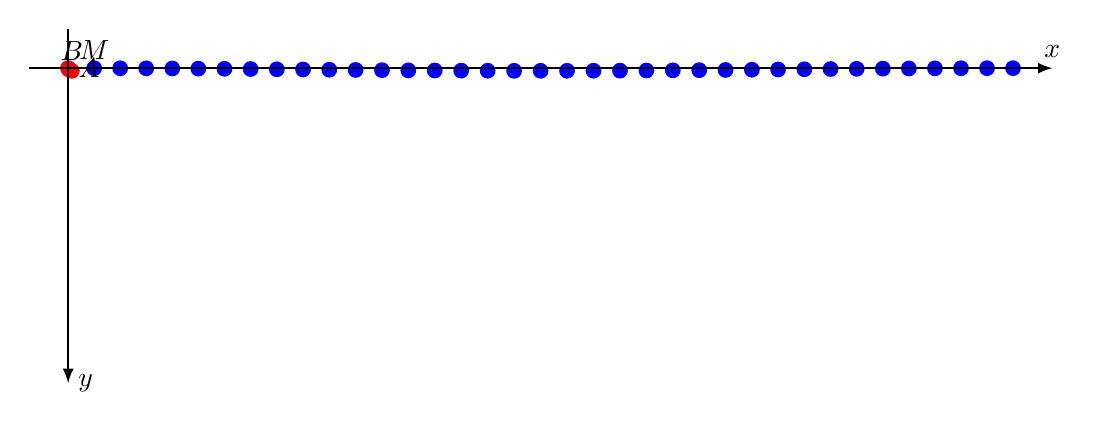
\begin{tikzpicture}[>=latex,thick]

	\begin{scope}
		\clip (-0.5,0.5) rectangle (12.3,{-2*\r-0.5});
		\foreach \p in {2,3,...,38}{
			\uncover<\p>{
				\kreis{(10*(\p-2))}
			}
		}
	\end{scope}

	\draw[color=red!50!black,line width=1.2pt]
		plot[domain=0:360,samples=100]
			({\r*3.1415*\x/180-\r*sin(\x)},{\r*(cos(\x)-1)});
	\draw[color=red,line width=2pt]
		plot[domain=40:170,samples=100]
			({\r*3.1415*\x/180-\r*sin(\x)},{\r*(cos(\x)-1)});

	\def\x{40}
	\fill[color=red]
		({\r*3.1415*\x/180-\r*sin(\x)},{\r*(cos(\x)-1)})
			circle[radius=0.1];
	\node at 
		({\r*3.1415*\x/180-\r*sin(\x)},{\r*(cos(\x)-1)})
			[right] {$A$};
	\def\x{170}
	\fill[color=red]
		({\r*3.1415*\x/180-\r*sin(\x)},{\r*(cos(\x)-1)})
			circle[radius=0.1];
	\node at 
		({\r*3.1415*\x/180-\r*sin(\x)},{\r*(cos(\x)-1)})
			[above] {$B$};


	\def\x{100}
	\fill[color=red]
		({\r*3.1415*\x/180-\r*sin(\x)},{\r*(cos(\x)-1)})
			circle[radius=0.1];
	\node at 
		({\r*3.1415*\x/180-\r*sin(\x)},{\r*(cos(\x)-1)})
			[above right] {$M$};
	\draw[->] (-0.5,0) -- (12.5,0) coordinate[label={$x$}];
	\draw[->] (0,0.5) -- (0,-4) coordinate[label={right:$y$}];
\end{tikzpicture}
\end{center}
\begin{quote}
Neue Aufgabe, zu deren Lösung die Mathematiker eingeladen werden.
Gegeben zwei Punkte $A$ und $B$ in einer vertikalen Ebene, finde
die Bahn $AMB$ eines Punktes $M$, der unter der Wirkung seines Gewichtes
in kürzester Zeit vom Punkt $A$ zum anderen Punkt $B$ absteigt.
\end{quote}
\end{frame}
\egroup
